\documentclass{homework}

\title{CHAPTER 1}
\author{1184100 MUH AMRI IRIANTO}

\begin{document}

\maketitle{SOAL CHAPTER 1 TEORI}

\section{TEORI UMUM}
\subsection{ Definisi, Sejarah dan perkembangan Kecerdasan Buatan}
\subsubsection{Definisi AI}
Kecerdasan buatan atau intelegensi artifisial dalam bahasa Inggris: Artificial Intelligence (AI) merupakan kecerdasan yang dimasukkan ke suatu sistem dan bisa diatur dalam konteks ilmiah.
Terdapat beberapa pengertian kecerdasan buatan atau artificial intelligence (AI) dalam berbagai sudut pandang.

\text Kecerdasan bauatan dalah usaha untuk memodelkan proses berfikir manusia dan mendesain mesin agar dapat menirukan perilaku manusia 
Kecerdasan bauatan juga suatu penelitian,aplikasi dan intruksi yang terkait dengan pemograman computer dalam melakukan suatu kegiatan menurut pandangan manusia

\subsubsection{Sejarah}
Dimulai pada tahun 1940 pada era computer elektronik benih-benih kecerdasan buatan ditanama kan oleh para filsuf klasik yang ingin menggabarkan proses berfikir manusia sebagai manipulasi dengan cara mekanis pada tahun 1940-an sebuah mesin yang disasarkan perangkat meginspirasi segelintir ilmuan untuk mulai serius untuk membangun sebua otak electronic.  

Istilah kecerdasan buatan pertaman kali dikemukakan pada 1956 di konfrensi Dartmouth, sejak itu kecerdasan hbuatan terus dikembangkan sebagai penelitian uuntuk teori-teori dan juga berkembangnya proinsip, Walaupun seperti itu istilah kecerdasan baru muncul pada tahun 1956 tetapi teori kecerdasan buatan sudah muncul sejak 1941

\subsubsection{Pekembangan}
Zaman computer Electronik (1941)

\text Pada tahun 1941 alat penyimpana dan pemrosesan informasi Ditemukan penemuan tersebut dinamakan Komputer electronic yang Dikembanghkan USA dan jerman. Saat itu computer melibatkan ribuan kabel untuk menjalankan suatu program.

Masa Awal Persiapan AI (1943-1956)

\text Tahun 1943 Warren McCulloch dan Walter Pitt mengemukakan tiga hal :
Pengetahuan fisiologi dasar dan fungsi sel syaraf dalam otak,analisis tengtang logika proposisi, dan teori komputasi turing mereka mamabuat midel sel sayaraf tiruan dimana setiap sel syaraf digambarkan dengan ON dan OFF menunjukkan bahawa setiap fungsi dapat dihitung  dengan suatu sel syaraf dans emua dapat di implemetasikan secara logis

\text tahun 1950, Nobert Wiener membuat penelitian mengenai prinsip-prinsip teori feedback. Contoh yang terkenal adalah thermostat. Penemuan ini juga merupakan awal dari perkembangan AI.
 
\text tahun 1956, John McCarthy meyakinkan Minsky, Claude Shannon dan Nathaniel Rochester untuk membantunya melakukan penelitian dalam bidan Otomata, Jaringan Syaraf dan pembelajaran intelijensia. Mereka mengerjakan proyek ini selama 2 bulan di Dartsmouth. Hasilnya adalah program yang mampu berpikir non-numerik dan menyelesaikan masalah pemikiran, yang dinamakan Principia Mathematica. Hal ini menjadikan McCarthy disebut sebagai bapak kecerdasan buatan.

Awal Perkembangan AI (1952-1969)

\text Pada tahun-tahun pertama perkembangannya, kecerdasan buatan mengalami banyak kesuksesan. Diawali dengan kesuksesan Newell dan Simon dengan ssebuah program yang disebut General Problem Solver.

\text Pada tahun 1958, McCarthy di MIT AI Lab Memo No.1 mendefinisikan bahasa pemrograman tingkat tinggi yaiyu LISP, yang sekarang mendominasi pembuatan program-pogram kecerdasan buatan. Kemudian, McCarthy membuat program yang dinamakan Programs with Common Sense. Di dalam program tersebut, dibuat rancangan untuk menggunakan pengetahuan dalam mencari solusi.

\text Pada tahun 1959, Nathaniel Rochester dari IBM dan mahasiswa-mahasiswanya mengeluarkan program kecerdasan buatan yaitu Geometry Theorm Prover. Program ini dapat mengeluarkan suatu teorema menggunakan aksioma-aksioma yang ada.

Sistem Berbasis Pengetahuan ( 1969 - 1979 )

\text Pengetahuan adalah kekuatan pendukung kecerdasan buatan. Hal ini dibuktikan dengan program yang dibuat oleh Ed Feingenbaum, Bruce Buchanan dan Joshua Lederberg yang membuat program untuk memecahkan masalah struktur molekul dari informasi yang didapatkan dari spectrometer massa.

Kembalinya Jaringan Syaraf Tiruan ( 1986 - Sekarang )

\text Meskipun bidang ilmu komputer menolak jaringan syaraf tiruan setelah diterbitkannya buku “Perceptrons” karangan Minsky dan Papert, para ilmuwan masih mempelajari bidang ilmu tersebut dari sudut pandang yang lain, yaitu fisika. Para ahli fisika seperti Hopfield (1982) menggunakan teknik-teknik mekanika statistika untuk menganalisia sifat-sifat penyimpanan dan optimasi pada jaringan syaraf. Para ahli psikologi, David Rumelhart dan Geoff Hinton, melanjutkan penelitian mengenai model jaringan syaraf tiruan pada memori.

\subsection{Definisi}
\subsubsection{supervise learning & unsupervise learning} supervise learning merupakan proses pegelompokan data yang telah memiliki labael dan akan dikelompokkan berdasarkan labelnya untuk mendapatkan label tertentu  untuk melakukan proses training terlebih dahulu.

unsupervised learning merupakan proses pengelompokan data yang tidak memiliki label. sehingga kita bebas meentukan jumlah kelompok data yang dibuat

\subsubsection{Klasifikasi dan Regresi}
\text klasifikasi dalah proses menemukan atau menemukan model (fungsi) yang membantu dalam memisahkan data menjadi beberapa kelas kategorikal.yang berrarti data yang dikategorikan dalam labe; yang berbeda sesuai dengan parameter

regresi adalah proses meneumkan model atau fungsi untuk emembedakan data menjadi nilai rill kotinu alih-alih menggunakna kelas secara matematis,dengan masalah regresi,sesorang berusaha menukan perkiraan fungsi dengan deviasi kesalahan minimun

\subsubsection{Dataset, Training Set dan Testing Set}
\text dataset istilah informar yang merujuk pada kumpulan data. secara umum dataset berisi lebih dari variable dan menyangkut satu topik: itu mungkin menyangkut satu sampel

Training set adalh bagian dari data set untuk memprediksi atau menjalankan fungsi dari sebuah algoritma ML. agar mesin yang kita latih mencari korelasi sendiri atau belajar denagn pola data yang diberikan

Testing set adalh bagian dataset yang kita tes untuk melihat keakuratannya atau dengan kata lain performanya



\section{IMPLEMENTASI}
untuk pertama kita bisa melakukan instalasi skit learn seperti gambar gambar dibawa melauli link
https://scikit-learn.org/stable/tutorial/basic/tutorial.html akan muncul juga tutorial mengenai penggunaan sckit learn 
\subsection{Instalasi Skit learn}
kita membuka anaconda prom terus kita bisa memasukkan 

\text conda create -n sklearn-env seperti gambar dibawah
\begin{center}
    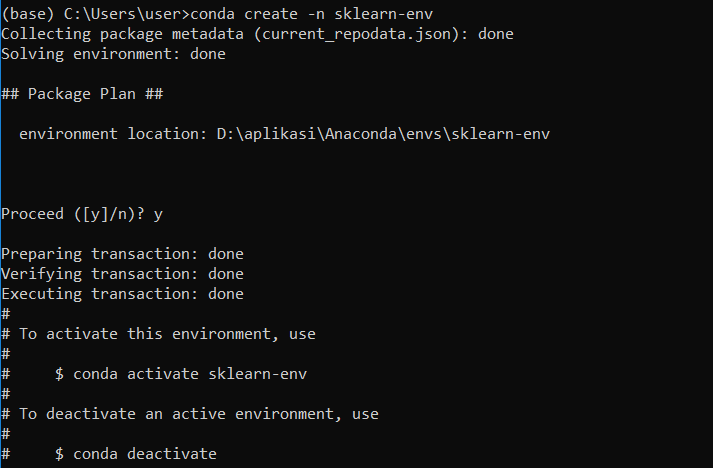
\includegraphics[width=.7\textwidth]{Figure/Instal1.PNG}
\end{center}

setelah itu kita bisa melakukan instalasi  seperti gambar dibawah untuk melihat apakah SCIKIT LEARN telah di instal
\begin{center}
    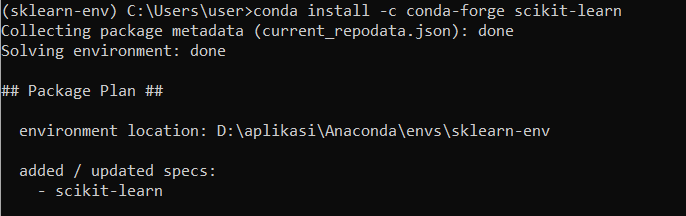
\includegraphics[width=.8\textwidth]{Figure/instal2.PNG}
\end{center}

Setelah itu,di harapkan melakuka pengecekan dengan conda seperti gambar dibawah
\begin{center}
    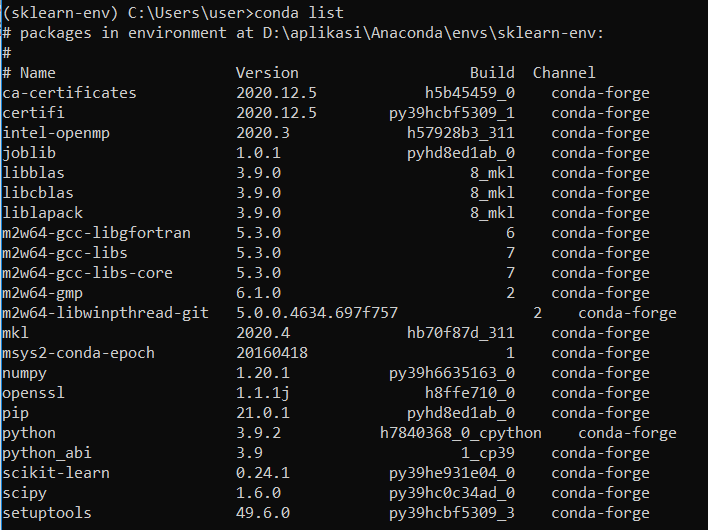
\includegraphics[width=.8\textwidth]{Figure/instal3.PNG}
\end{center}

\subsection{Loading an example dataset}
pada halaman ini kalan dilakukan test example data set untuk mengabil data pada scikit learn 
kita masukkan kode untuk melakukan test :

\begin{verbatim}
from sklearn import datasets
iris = datasets.load_iris()
digits = datasets.load_digits()
print(digits.data)
\end{verbatim}
maka hasilnya akan terliha seperti gambar dibawah 

\begin{center}
    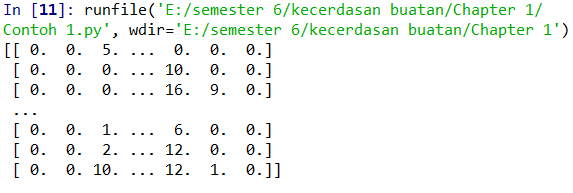
\includegraphics[width=.8\textwidth]{Figure/hasil1.PNG}
\end{center}

\subsection{Learning and predicting}
pada percobaaan kali ini kita akan menggunakan learning and predicting untuk melakukan prediksi dan penggunaan leraning langsung seperti contoh dibawah

\begin{verbatim}
from sklearn import datasets 
iris = datasets.load_iris()
digits = datasets.load_digits()
from sklearn import svm
clf = svm.SVC(gamma=0.001, C=100)
clf.fit(digits.data[:-1], digits.target[:-1])
hasil = clf.predict(digits.data[-1:])
print(hasil)
\end{verbatim}
maka hasilny akan seperti gambar dibawah:
\begin{center}
    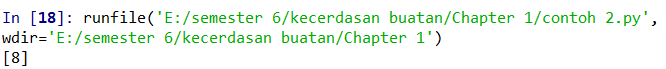
\includegraphics[width=.8\textwidth]{Figure/Hasil2.PNG}
\end{center}

\subsection{Model persistence}
pada tahap ini akan menggunakan model persintence untuk 
berikut kita bisa melihat seperti contoh dibawah untuk melakukan uji coba

\begin{verbatim}
from sklearn import svm
from sklearn import datasets
clf = svm.SVC()
X, y = datasets.load_iris(return_X_y=True)
clf.fit(X, y)

#pickle
import pickle 
s = pickle.dumps(clf)
clf2 = pickle.loads(s)
clf2.predict(X[0:1])
print(y[0])

#joblib
from joblib import dump, load
dump(clf, '1184100.joblib')
clf3 = load('1184100.joblib')
print(clf3.predict(X[0:1]))
\end{verbatim}
maka hasilnya akan seperti gambar dibawah 
\begin{center}
    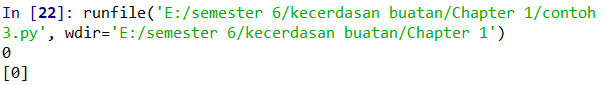
\includegraphics[width=.8\textwidth]{Figure/hasil3.PNG}
\end{center}

\subsection{Conventions}
scikit-learn estimator mengikuti aturan tertentu untuk membuat perilakunya lebih prediktif,
seperti contoh dibawah:

\begin{verbatim}
import numpy as np
from sklearn import random_projection

rng = np.random.RandomState(0)
X = rng.rand(10, 2000)
X = np.array(X, dtype='float32')
X.dtype

transformer = random_projection.GaussianRandomProjection()
X_new = transformer.fit_transform(X)
X_new.dtype
print(X_new)
\end{verbatim}
maka hasilnya akan seperti gambar dibawah
\begin{center}
    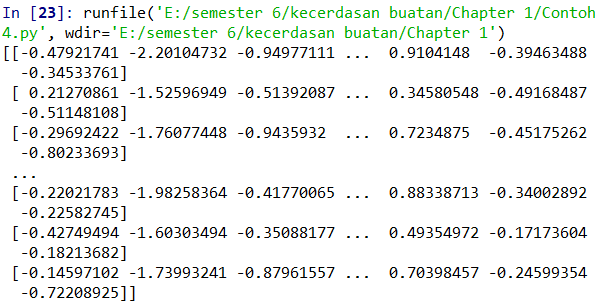
\includegraphics[width=.8\textwidth]{Figure/hasil4.PNG}
\end{center}

\section{Penanganan Erorr}

\begin{enumerate}
    \item pada eororr petama ditunjukkan found input yang salah pada input found variabel
\begin{center}
    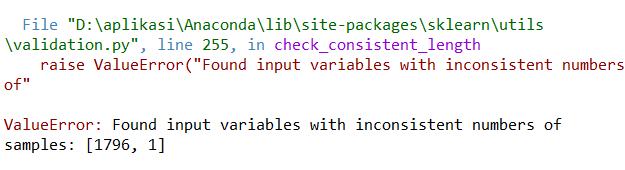
\includegraphics[width=.8\textwidth]{Figure/erorr1.PNG}
\end{center}    
    \item erorr kedua di tunjukaan pada input float sehingga varibale tidak dapat terbaca dan terjadinya errorr
\begin{center}
    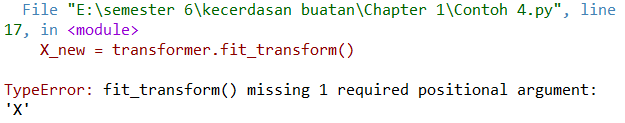
\includegraphics[width=.8\textwidth]{Figure/erorr2.PNG}
\end{center} 
\end{enumerate}
\end{document}
